% 2018 江苏 12 图：直线 l:y=2x；B(5,0)；以 AB 为直径的圆 C，圆心 C(4,3)，A(3,6)，D(1,2)。
% 全局数值坐标，单位 1cm，线宽 .6pt，12pt。
\usetikzlibrary{arrows.meta,calc}
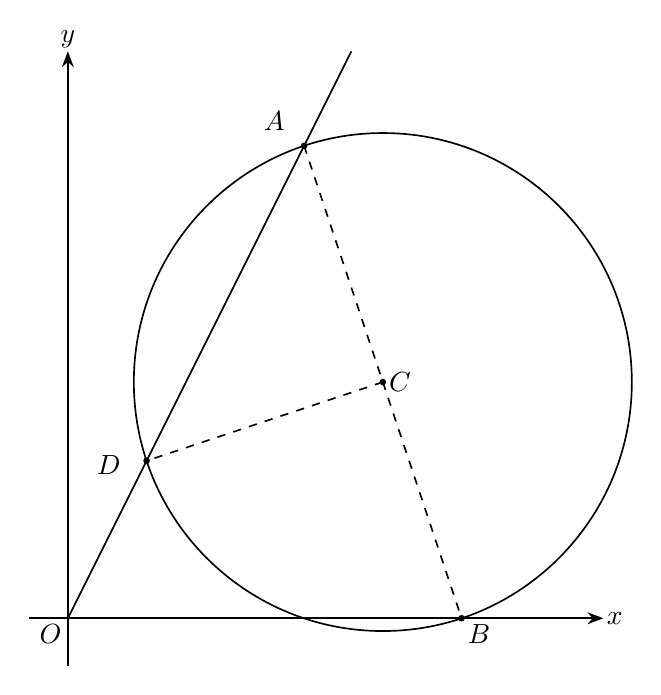
\begin{tikzpicture}[x=1cm,y=1cm,line width=.6pt,>=Stealth,font=\normalsize]
\coordinate (O) at (0,0);
\coordinate (A) at (3,6);
\coordinate (B) at (5,0);
\coordinate (D) at (1,2);
\coordinate (C) at (4,3);
\draw[->] (-0.5,0)--(6.8,0) node[right,inner sep=1pt] {$x$};
\draw[->] (0,-0.6)--(0,7.2) node[above,inner sep=1pt] {$y$};
\draw (C) circle [radius=3.162278cm];
\draw (O)--(3.6,7.2);
\draw[dashed] (A)--(C);
\draw[dashed] (C)--(D);
\draw[dashed] (C)--(B);
\fill (A) circle (1.2pt);
\fill (D) circle (1.2pt);
\fill (C) circle (1.2pt);
\fill (B) circle (1.2pt);
\node[inner sep=1pt] at (2.62,6.32) {$A$};
\node[anchor=north west,inner sep=0pt,xshift=2pt,yshift=-2pt] at (B) {$B$};
\node[anchor=west,inner sep=0pt,xshift=2pt] at (C) {$C$};
\node[inner sep=1pt] at (0.52,1.95) {$D$};
\node[anchor=north east,inner sep=0pt,xshift=-2pt,yshift=-2pt] at (O) {$O$};
\end{tikzpicture}
